\let\negmedspace\undefined
\let\negthickspace\undefined
\documentclass[journal,12pt,twocolumn]{IEEEtran}
\usepackage{cite}
\usepackage{amsmath,amssymb,amsfonts,amsthm}
\usepackage{algorithmic}
\usepackage{graphicx}
\usepackage{textcomp}
\usepackage{xcolor}
\usepackage{txfonts}
\usepackage{listings}
\usepackage{enumitem}
\usepackage{mathtools}
\usepackage{gensymb}
\usepackage[breaklinks=true]{hyperref}
\usepackage{tkz-euclide} % loads  TikZ and tkz-base
\usepackage{listings}
\usepackage{gvv}
\usepackage{amsmath}

        

\newtheorem{theorem}{Theorem}[section]
\newtheorem{problem}{Problem}
\newtheorem{proposition}{Proposition}[section]
\newtheorem{lemma}{Lemma}[section]
\newtheorem{corollary}[theorem]{Corollary}
\newtheorem{example}{Example}[section]
\newtheorem{definition}[problem]{Definition}
\newcommand{\BEQA}{\begin{eqnarray}}
\newcommand{\EEQA}{\end{eqnarray}}
\newcommand{\define}{\stackrel{\triangle}{=}}
\theoremstyle{remark}
\newtheorem{rem}{Remark}

%\bibliographystyle{ieeetr}
\begin{document}
%

\bibliographystyle{IEEEtran}


\vspace{3cm}

\title{
%	\logo{
Assignment-2

\large{EE1205 : Signals and Systems}

Indian Institute of Technology Hyderabad
%	}
}
\author{Chirag Garg

(EE23BTECH11206)
}	





\maketitle

\newpage



\bigskip

\renewcommand{\thefigure}{\theenumi}
\renewcommand{\thetable}{\theenumi}


\section{Question 11.9.1 (5)}
\vspace{0.5cm}
\begin{flushleft}
 Write the first five terms of the sequence whose $n^{th}$ \text{term is} : $x(n) = (-1)^{n-1}5^{n+1}$.
\end{flushleft} 


\vspace{0.8cm}


\section{Solution} 






To find the $Z$-transform of a sequence, we use the formula:
\begin{align}
X(z) = \sum_{n=0}^{\infty} x[n] \cdot z^{-n} 
\end{align}

Given the sequence $a_n = (-1)^{n-1} \cdot 5^{n+1}$, we can substitute this into the formula:
\begin{align}
A(z) &= \sum_{n=0}^{\infty} (-1)^{n-1} \cdot 5^{n+1} \cdot z^{-n} \\ 
 &= \sum_{n=0}^{\infty} (-1)^{n-1} \cdot \frac{5^{n+1}}{z^n} 
\end{align}
Now, let's split the summation into two parts, one for even values of $n$ and one for odd values of $n$:
\begin{align}
 A(z) &= \sum_{n=0}^{\infty} (-1)^{n-1} \cdot \frac{5^{n+1}}{z^n} \\
  &= \sum_{k=0}^{\infty} (-1)^{2k-1} \cdot \frac{5^{2k+1}}{z^{2k}} + \sum_{k=0}^{\infty} (-1)^{2k} \cdot \frac{5^{2k+2}}{z^{2k+1}} \\
 &= -\sum_{k=0}^{\infty} \frac{5^{2k+1}}{z^{2k}} + \sum_{k=0}^{\infty} \frac{5^{2k+2}}{z^{2k+1}} \\
&= -5\sum_{k=0}^{\infty} \left(\frac{5}{z}\right)^{2k} + 5\sum_{k=0}^{\infty} \left(\frac{5}{z}\right)^{2k+1} \\
&=\dfrac{-5}{1 - 25 \times z^{-2}} + \dfrac{25 \times z^{-1}}{1 - 25 \times z^{-2}} \\
&=\dfrac{-5 \times z}{z+5} \\
\end{align}

This result is valid for R.O.C. $\left| \dfrac{5 }{ z }\right| < 1$ \\
\begin{align}
|z| > 5
\end{align}



\begin{figure}
  \centering
  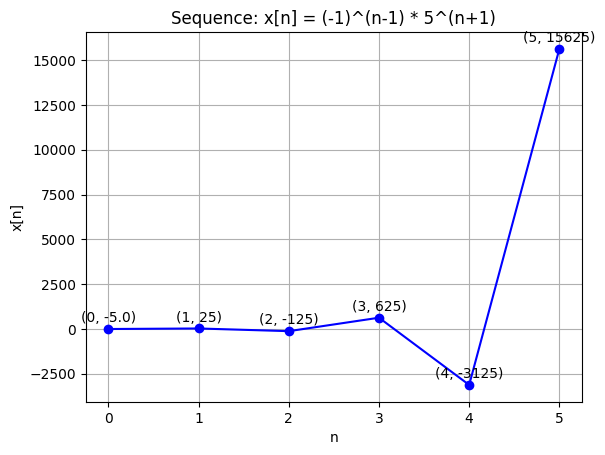
\includegraphics[width=0.5\textwidth]{grasi2.png} 
 
\end{figure}

The $Z$-transform of the given sequence $a_n$ is $A(z)$ as derived above.




















The $n^{th}$ term of sequence is: $x(n) = (-1)^{n-1}5^{n+1}$\\
On substituting n = 0, 1, 2, 3 and 4, we get the first five terms 

Hence, the required terms are -5, 25, –125, 625, –3125 .


\end{document}